\documentclass[11pt]{article}
% Manejo del idioma español                           
\usepackage[spanish]{babel}
\usepackage{geometry}
\geometry{
  paperheight=297mm,
  paperwidth=210mm,
  left=30mm,
  right=20mm,
  top=10mm,
  bottom=10mm}

\usepackage{hyperref}
\hypersetup{
  pdftitle=Catorce preceptos de vida,
  pdfauthor=Thich Nhat Hanh,
  pdfsubject=Extraído del libro “Puerta a la compasión”,
  pdfkeywords=mindfulness,
  %pdfproducer=,
  pdfcreator=XeLaTeX}

\usepackage{wallpaper}  
%for loading fonts
\usepackage{fontspec}  
\setmainfont[
  Path = fonts/,
  BoldFont = AGaramondPro-Bold,
  BoldItalicFont = AGaramondPro-BoldItalic,
  ItalicFont = EBGaramond12-Italic,
  SmallCapsFont = EBGaramond12-SC]{EBGaramond12-Regular}
  
%--------------------BEGIN DOCUMENT----------------------
\begin{document}
\thispagestyle{empty}
\ThisCenterWallPaper{1}{bamboo.pdf}

{\noindent\em No creas que yo siento que sigo todos y cada uno de estos preceptos perfectamente. Sé que fallo de muchas maneras. Ninguno de nosotros puede cumplir plenamente cualquiera de ellos. Sin embargo, debo trabajar hacia una meta. Esta es mi meta. Ninguna palabra puede reemplazar a la práctica, sólo la práctica puede hacer a las palabras.}

\begin{description}
\item[Se abierto en tus ideas o teorías.] No seas idólatra ni te ates a ninguna doctrina, teoría o ideología. Todos los sistemas de pensamiento son medios de guía; no son la verdad absoluta.

\item[Encuentra tu verdad en la vida, pero permítete cambiar.] No creas que el conocimiento que tienes en este momento es la verdad inmutable, absoluta. Evita ser de mentalidad estrecha y atarte a los puntos de vista presentes. La verdad se encuentra en la vida y no meramente en el conocimiento conceptual.

\item[Renuncia al fanatismo y ayuda a otros a que también lo hagan.] No fuerces a los demás, ni siquiera a los niños, por ningún medio en absoluto, a adoptar tus puntos de vista, ya sea por autoridad, amenaza, dinero, propaganda o incluso educación. Sin embargo, por medio del diálogo compasivo, ayuda a los demás a renunciar al fanatismo y la estrechez.

\item[Despiértate a la realidad y el sufrimiento del mundo.] No evites el contacto con el sufrimiento ni cierres tus ojos ante el sufrimiento. No pierdas la conciencia de la existencia del sufrimiento en la vida del mundo. Despierta tú mismo y a los demás a la realidad del sufrimiento en el mundo.

\item[Comparte lo que tienes y busca trascender más allá de lo material] No tomes como el objetivo de tu vida a la fama, el provecho, la riqueza o el placer sensual. Vive simplemente y comparte el tiempo, la energía y los recursos materiales con quienes están en necesidad.

\item[Practica la compasión.] No mantengas ira u odio. Tan pronto como surgen la ira y el odio, practica la meditación sobre la compasión para comprender profundamente a las personas que han causado ira y odio. Aprende a ver a los otros seres con los ojos de la compasión.

\item[Practica la respiración, la atención y la comprensión.] No te pierdas en la dispersión y en el ambiente que te rodea. Aprende a practicar la respiración para recuperar la compostura del cuerpo y la mente, para practicar la atención, y para desarrollar la concentración y la comprensión.

\item[Usa palabras conciliadoras y resolutivas.] No pronuncies palabras que puedan crear discordia y causar ruptura en la comunidad. Haz todos los esfuerzos para reconciliar y resolver todos los conflictos, aunque sean pequeños.

\item[Asiente a la verdad y a la justicia, con sinceridad y discreción.] No digas cosas falsas por el bien del interés personal o para impresionar a las personas. No critiques o condenes cosas de las que no estás seguro. Habla siempre verdadera y constructivamente. Ten el valor de hablar sobre situaciones de injusticia, aun cuando hacerlo pueda amenazar tu propia seguridad.

\item[No uses a los demás para tu provecho personal.] No transformes tu comunidad en un partido político, ni la uses para tu ganancia o provecho personal. Toma una actitud clara contra la opresión y la injusticia, sin engancharte en conflictos partidarios.

\item[Elige una vocación amorosa.] No vivas con una vocación que sea dañina para los humanos y la naturaleza. No inviertas en compañías que priven a los demás de su oportunidad de vivir. Elige una vocación que ayude a realizar tu ideal de compasión.

\item[Protege la vida.] Encuentra todos los medios posibles para proteger la vida y prevenir la guerra.

\item[Respeta la propiedad y evita que los demás se enriquezcan con el sufrimiento humano.] No poseas nada que debería pertenecer a los demás. Respeta la propiedad de los demás pero evita que los demás se enriquezcan con el sufrimiento humano o el sufrimiento de otros seres.

\item[Cuida tu cuerpo y no lo veas como un instrumento.] No maltrates a tu cuerpo. Aprende a manejarlo con respeto. No veas a tu cuerpo sólo como un instrumento. Respeta los derechos y compromisos de los demás.
\end{description}

\medskip
\raggedleft{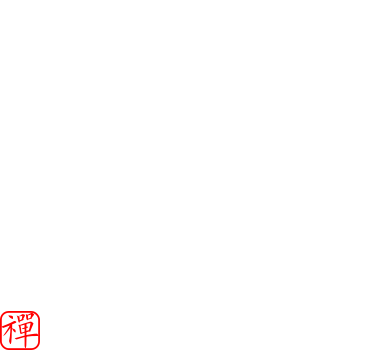
\includegraphics[scale=1.3]{hanko.pdf} ~~~~~~~~~~~~~~~~~~\\
\large\sc Thích Nhâ\kern-.27em´\kern-.15emt Hạnh} ~~~~~
\end{document}
